\section{System Design}
\label{sec:design}

\begin{figure*}[t]
  \centering
  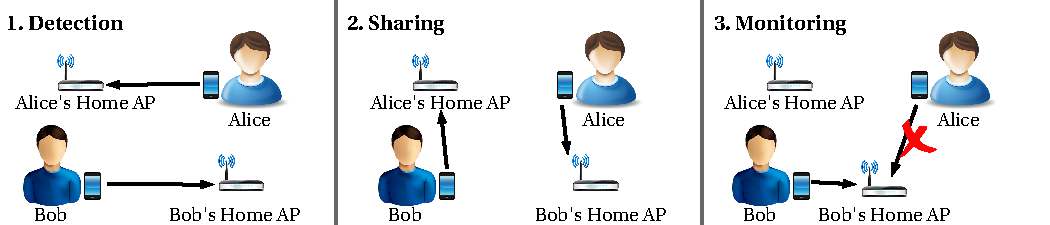
\includegraphics[width=\textwidth]{./figures/design.pdf}
  \caption{\textbf{\wisefi{} System Work Flow.}}
  \label{fig:design}
\end{figure*}

Inspired by the results of the investigation in Section~\ref{sec:investigation},
we design a system called \wisefi{} to detect reciprocal sharing
opportunities (\S\ref{subsec:detection}), enable \wifi{} sharing
(\S\ref{subsec:sharing}) and monitor the \wifi{} performance to ensure the
sharing remains reciprocal (\S\ref{subsec:monitoring}). Figure~\ref{fig:design}
shows the overall work flow of the \wisefi{} system.

\subsection{Detection}
\label{subsec:detection}

To detect reciprocal sharing opportunities, two information are required: the
home AP of the device, and neighbor APs' signal strength during \wifi{} sessions
with the home AP. A smartphone application will be deployed through app market
to collect these information. In particular, the home AP information can be
learned over a period of time using the heuristics developed in
Section~\ref{subsec:homeap}, or be resolved through user input. \wifi{} scan
results during sessions with home APs can then be logged to identify the
neighbor APs that can potentially provide better signal. Finally, these
information are uploaded and fused in \wisefi{} server to identify reciprocal
sharing opportunities as described in Section~\ref{subsec:reciprocal}.

\subsection{Sharing}
\label{subsec:sharing}

Once the reciprocal sharing opportunities are discovered, the \wisefi{} server
can then distribute such information to the smartphone clients, which will
prompt users to establish \wifi{} sharing. The sharing mechanism must meet two
goals: control and protection. First, the system should be able to control the
sharing, including granting the access of home AP to other \wisefi{} users, and
revoking the access when the reciprocal sharing opportunity no longer exists.
Second, the system should protect the home network from other \wisefi{} users by
sharing access only to the Internet, and protecting private resources such as
network printer or home network storage.

For home APs which support virtual guest network feature, the \wifi{} sharing
can be achieved by only distributing the credential of guest network to other
\wisefi{} users. Access and traffic policies can then be enforced on the guest
network to achieve control and protection. For APs without guest network
feature, however, cumbersome AP configurations may be required, such as MAC
black or white list, routing table entry. Such configurations are probably too
complicated for average users to perform. We discuss possible solutions in
Section~\ref{sec:challenges}.


\subsection{Monitoring}
\label{subsec:monitoring}

After the sharing is established, the system needs to monitor the \wifi{}
performance to ensure that the sharing remains reciprocal. There are two
reasons. First, as mentioned in Section~\ref{subsec:better}, the system uses
signal strength as a hint to identify potentially better APs. And it is well
known that signal strength does not directly translate to \wifi{} performance.
Other factors, such as AP load, modulation, interference, or \wifi{} generation,
which can not be easily detected by the smartphone, also affect the link
quality. Furthermore, last hop \wifi{} link quality does not necessarily
determines the overall end-to-end network performance. Therefore, whether
connecting to neighbor AP can indeed improve the user's network performance is
unknown until the sharing is actually established. Second, it is important to ensure that
the sharing remains reciprocal in long terms for fairness concerns. For
instance, a \wisif{} user may have a new AP deployed at home such that the home APs
always provide better or comparable \wifi{} coverage than the neighbor APs, and
there are no longer needs to share neighbor APs. The system should be able to
detect the termination of the reciprocal sharing relationship and revoke the
peer's access to the user's home AP.

